\documentclass[11pt]{article}
\usepackage{graphicx}
\usepackage{amsmath, amssymb, amsthm}
\usepackage{amsfonts}
\usepackage{geometry}
\usepackage{epstopdf}
\usepackage{bbm}
\usepackage{subcaption}
\usepackage{color}
\usepackage[toc,page]{appendix}
%\usepackage{subfigure}
%\documentclass{acm_proc_article-sp}
\usepackage{setspace}
\usepackage{enumerate}
\usepackage{algorithm}
\usepackage{algorithmic}
\newtheorem{theorem}{Theorem}
\newtheorem{assumption}{Assumption}
\renewcommand{\thetheorem}{ \arabic{theorem}}
\newtheorem{corollary}[theorem]{Corollary}
\renewcommand{\thecorollary}{\arabic{corollary}}
\newtheorem{definition}{Definition}
\renewcommand{\thedefinition}{\arabic{definition}}
\newtheorem{lemma}{Lemma}

\newcommand{\E}{\mathbb{E}}
\newcommand{\argmax}{\operatornamewithlimits{argmax}}
\newcommand{\argmin}{\operatornamewithlimits{argmin}}
\newcommand{\KG}{\mathrm{KG}}
\newcommand{\KGs}{\mathrm{KG}}
\newcommand{\KGp}{\mathrm{KG}^2}
\newcommand{\nuKGp}{\nu^{KG2}}
\newcommand{\zap}[1]{}
\newcommand{\twovec}[2]{\left( \begin{array}{c}#1\\ #2\end{array} \right)}
\newcommand{\twomatrix}[4]{\left(\begin{array}{cc}#1&#2\\#3&#4\end{array}\right)}
\newcommand{\Prob}{\mathbb{P}} % probability measure
\newcommand{\e}[1]{\left\{#1\right\}}
\newcommand{\s}[1]{\left[ #1 \right]}
\newcommand{\length}{\mathrm{length}}
\newcommand{\Ytilde}{\widetilde{Y}}
\newcommand{\Fn}{\mathcal{F}_n}
\newcommand{\Ncal}{\mathcal{N}}
\newcommand{\Var}{\mathrm{Var}}
\newcommand{\R}{\mathbb{R}}
\newcommand{\N}{\mathbb{N}}
\newcommand{\Z}{\mathbb{Z}}
\newcommand{\lsb}{\left[}
\newcommand{\rsb}{\right]}
\newcommand{\lp}{\left(}
\newcommand{\sigmatilde}{\tilde{\sigma}}
\newcommand{\rp}{\right)}
% \newcommand{\xvec}{{\bf x}}
% \newcommand{\Yvec}{{\bf Y}}
\newcommand{\xvec}{x}
\newcommand{\Yvec}{Y}

\newcommand{\figref}[1]{Figure~\ref{#1}}
\newcommand{\secref}[1]{\S\ref{#1}}     % NB: Still sshould write Section~\ref{ABC} at start of a sentence
\newcommand{\secrefb}[2]{\S\ref{#1}-\S\ref{#2}}

\newcommand{\omg}{\omega}
\newcommand{\sv}{\mathbf{s}}
\newcommand{\Sv}{\mathbf{S}}
\newcommand{\av}{\mathbf{a}}
\newcommand{\bv}{\mathbf{b}}
%\newcommand{\cv}{\mathbf{c}}
\newcommand{\cv}{c}
%\newcommand{\dv}{\mathbf{d}}
\newcommand{\dv}{d}
\newcommand{\muv}{\pmb{\mu}}
\newcommand{\betav}{\pmb{\beta}}
%\newcommand{\thetav}{\pmb{\theta}}
\newcommand{\thetav}{\theta}
\newcommand{\lambdav}{\pmb{\lambda}}
\newcommand{\alphav}{\pmb{\alpha}}
%\newcommand{\thetav}{\theta}
\newcommand{\NoGa}{\mathcal{NG}}
\newcommand{\zv}{\mathbf{z}}
\newcommand{\wv}{\mathbf{w}}
\newcommand{\ev}{\mathbf{e}}
\newcommand{\piv}{\pmb{\pi}}
\doublespacing

\usepackage{url}
    \title{Perovskite Model Description}
\begin{document}
\newcommand{\hwccomment}[1]{{\color{red} (#1)}}
\maketitle
\section{Introduction}
In this project we are interested in finding a perovskite composite with the highest unsaturated Mayer Bond order (UMBO). We approach this problem with Bayesian Optimization. This documentation provides model description of the single-halide scenario and presents results obtained by using the model.
\section{Single-halide Model}
\subsection{Model setup}
In a single-halide model, the setup contains one halide, one cation and one solvent. There are 3 choices for halides, 3 for cations and 8 for solvents, hence 72 possible setups in total. Let $V_x$ to denote the value (UMBO) of setup $x$, $x\in \{1,...,72\}$. We use vector $Z^x$ to describe the components of setup $x$, with each index $i$ corresponding to a possible element in the setup. In particular, $Z^x_i, i\in\{1,2,3\}$ is a binary variable that indicates whether a cation is present in setup x. We require that $\sum_{i=1}^3Z^x_i=1, \forall x$, since there is only one cation present in each setup. Likewise, $Z^x_i, i\in\{4,5,6\}$ is a binary variable that indicate whether a halide is present in setup x. $Z_7^x \in \{s_1,...,s_8\}$ indicates which solvent is used in setup $x$. For example, $Z^x = (1,0,0,0,1,0,s_{4})$ means that setup $x$ contains the first type of cation, second type of halide, and the $4^{th}$ type of solvent. In addition, for future computation, we let $s_i$ be a 2-d vector with the first entry being the MVEE and the second entry being the polarity of the $i^{th}$ solvent, $i\in\{1,...,8\}$. 

We assume the presence of cations and halides contributes linearly to the objective value, and we use $\alpha_i$ to quantify the amount contributed by cation/halide $i$. To correct for the possible non-linear effects of cations and halides, we introduce $\beta_x$ for each of the setup x. For solvents, we assume they affect the solubility through an unknown function $f:\mathbb{R}^{2}\mapsto \mathbb{R}$ which takes into consideration the MVEE and polarity of a solvent. In addition to just a halide, a cation and a solvent, a perovskite also contains a central ion, for which we choose lead for all compositions. We use $\zeta$ to denote the contribution of the central ion to the objective function. Hence solubility of setup $x$ can be written in the following way:
\begin{equation}
V_x = \sum_{i=1}^{6}\alpha_i Z_i^x + \beta_x + \zeta + f(Z_7^x).
\end{equation}
We place the same prior distribution $N(\mu_{\alpha},\sigma^2_{\alpha})$ on each of $\alpha_i$, and $N(0, \sigma^2_{\beta})$ on $\beta_x$. $\zeta$ is assume to follow $N(\mu_{\zeta}, \sigma^2_{\zeta})$ According to the  Bayesian approach we suppose that $f(\cdot)$ is drawn from a Gaussian process with prior mean function $\mu_0(\cdot)$ and covariance $\Sigma_0(\cdot,\cdot)$. Since $\zeta$ already captures the invariant contribution from the central ion, it is reasonable for us to assume $\mu_0(\cdot)=\mathbf{0}$. We assume that two setups will have similar objective values if they differ little in their parts. To formalize this, for $\Sigma_0(\cdot,\cdot)$, we use 5/2 Mat\'ern kernel. Let $r = \sqrt{\sum_{i=1}^{d}\ell_i(x_{1,i}-x_{2,i})^2}$ denote the distance between point $x_1$ and $x_2$ weighed by each dimension. In our case $d = 2$. The covariance between $x_1$ and $x_2$ under a 5/2 Mat\'ern kernel is calculated as:
\begin{equation}
\Sigma_0(x_1,x_2) =  \sigma_m^2\left(1+\sqrt{5}r+\frac{1}{3}5r^2
\right)exp\left(-\sqrt{5}r\right),
\end{equation}
where $\sigma^2_m, \ell_i$ are hyper-parameters. With all the components of $V_x$ being normally distributed, $V_x$ is also normally distributed. Hence we are able to describe the joint distribution of $(v_1,...,v_{27})$ with a multivariate normal distribution:
\begin{equation}\label{prior}
\begin{pmatrix}
V_1 \\ V_2 \\ \vdots \\ V_{135}
\end{pmatrix} \sim N\Large(\mu^0, \Sigma^0\Large),
\end{equation}
where 
\begin{align*}
\mu^0_x &= \mathbb{E}\left[\sum_{i=1}^{6}\alpha_i Z_i^x + \beta_x + \zeta + f(Z_7^x)\right]\\
& = \sum_{i=1}^{6} \mu_{\alpha}Z^x_i+\mu_{\zeta}+\sum_{i=1}^{15}\mathbbm{1}(Z_7^x=s_i)\mu_{0,i}\\
& = 2\mu_{\alpha} + \mu_{\zeta},
\end{align*}
and
\begin{align*}
\Sigma^0_{x,x'} &= COV(V_x,V_{x'})\\
& =\sum_{i=1}^{6}\sigma_{\alpha}^2\mathbbm{1}(Z_i^{x}=1)\mathbbm{1}(Z_i^{x'}=1) + \Sigma_0(Z^x_7,Z^{x'}_7) + \mathbbm{1}(x=x')\sigma_{\beta}^2 + \sigma^2_{\zeta}
\end{align*}
\subsection{Estimation of Hyper-parameters}
We estimate the hyper-parameters by maximum likelihood estimation method. Let $\theta = \{\mu_{\alpha},\sigma_{\alpha}, \sigma_{\beta},\mu_{\zeta}, \sigma_{\zeta}, \ell_1, \ell_2\}$ be the vector of all the hyper-parameters we want to estimate. Let $V = \{v_{i_1},...,v_{i_m}\}$ to be the observations we made for $i_1,...,i_m$. Then the likelihood of $V$ given $\theta$ is 
\begin{align*}
L(\theta) &= P(V|\theta) \\
&= (2\pi)^{-m/2}*|\Sigma^0(i_1,...,i_m)|*\exp\left(-\frac{1}{2}u^0(i_1,...,i_m)^T\Sigma^0(i_1,...,i_m)u^0(i_1,...,i_m)\right),
\end{align*}
where $u^0(i_1,...,i_m) = (u^0_{i_1},...,u^0_{i_m})$ is a vertical vector, and $\Sigma^0(i_1,...,i_m)u^0(i_1,...,i_m)$ is a $m \times m$ matrix with $\{k,j\}$ entry = $\Sigma^0_{i_k, i_j}$.

The MLE of $\theta$ is set to be
\begin{equation}\label{mle}
\hat{\theta} = \argmax_{\theta}\hspace{1mm}log(L(\theta)).
\end{equation}
A maximizer of \eqref{mle} can be found via gradient-based optimization algorithms such as BFGS.  
\subsection{Posterior update}
We can update the mean and covariance in \eqref{prior} after we make an observation. Let $\mu^n$ and $\Sigma^n$ denote the mean and covariance in \eqref{prior} after $n$ observations are made. It is a well known fact that we can update the posterior distribution in the following way: given $\mu^n$ and $\Sigma^n$, and a new observation $\hat{y}^{n+1}$ which is made about setup $x$, the new posterior is:
\begin{equation}
\mu^{n+1} = \mu^n + \frac{\hat{y}^{n+1}-\mu_x^n}{\Sigma_{xx}^n}\Sigma^n\mathbf{e}_x,
\end{equation}
\begin{equation}
\Sigma^{n+1} = \Sigma^{n} - \frac{\Sigma^n\mathbf{e}_x \mathbf{e}_x^T\Sigma^n}{\Sigma_{xx}^n}
\end{equation}
\subsection{Choosing the next composition to be studied}\label{sec:sinEI}
Expected Improvement (EI) is used to determine which setup $x$ the next observation is to be made.
Let $\hat{y}^* = \max_{1,...,n}\{\hat{y_1},...,\hat{y_n}\}$ be the largest observed value so far. Assuming a maximizing problem, the expected improvement (EI) of a setup $x$ is:
\begin{align*}
EI(x) & = \mathbb{E}\Big[\max\{V_x - \hat{y}^*, 0\}\Big|\mu^n, \Sigma^n \Big] \\
& = (\mu_{x}^{n} - \hat{y}^*)\Phi\left(\frac{\mu_{x}^{n} - \hat{y}^*}{(\Sigma_{xx}^n)^{1/2}}\right) + (\Sigma_{xx}^n)^{1/2}\phi\left(\frac{\mu_{x}^{n} - \hat{y}^*}{(\Sigma_{xx}^n)^{1/2}}\right),
\end{align*}
where $\Phi(\cdot)$ and $\phi(\cdot)$ are standard normal cdf and pdf respectively.

We pick the setup with the largest $EI$:
\begin{equation}
x^* = \argmax_{x\in\{1,...,72\}}EI(x)
\end{equation}
\subsection{Experiment Result}
We first use leave-one-out cross validation to verify that our model fits the data well. 20 samples (compositions and their values) are selected randomly. Each time one sample is left out and hyperparameters of our model are estimated using the rest 19 samples. We then compare the values of the sample left out to the confidence interval of the value calculated based on the parameters estimated. Figure \ref{loo} plots the result of the cross validation. It can been seen that most of the observed value lies within the corresponding confidence interval, thus indicating a good fit of the model to the data.
\begin{center}
\begin{figure}
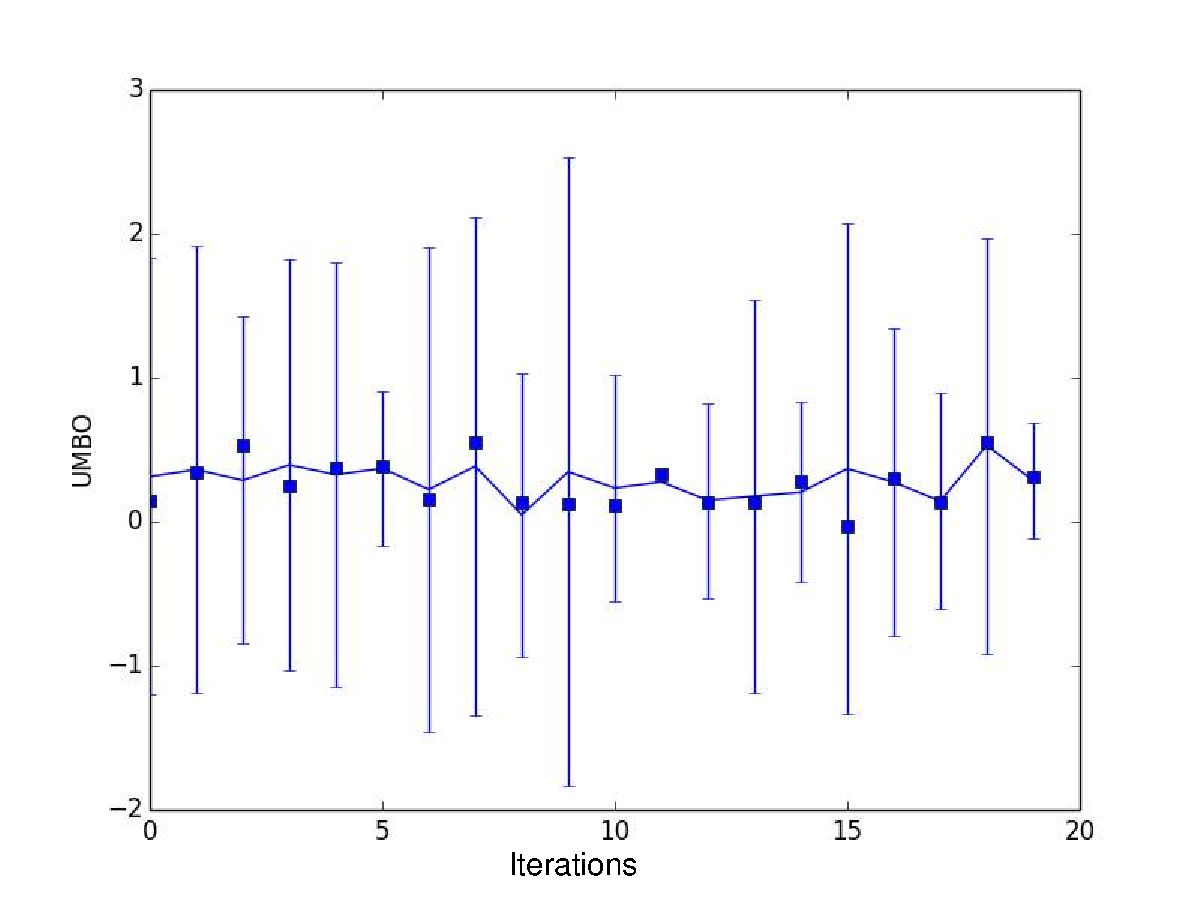
\includegraphics[scale=.8]{plot_loocv.pdf}
\caption{Plot of results of leave-one-out cross validation for 20 samples}
\label{loo}
\end{figure}
\end{center}
Figure \ref{plot_bo} plots the result of the sampling process by using the Bayesian optimization method aforementioned. The red line shows the true maximum value among all the possible setups. We can see that it takes 14 iterations for the BO process to converge to the true maximum, which is considerably less effort than carrying out the sampling randomly.
\begin{center}
\begin{figure}
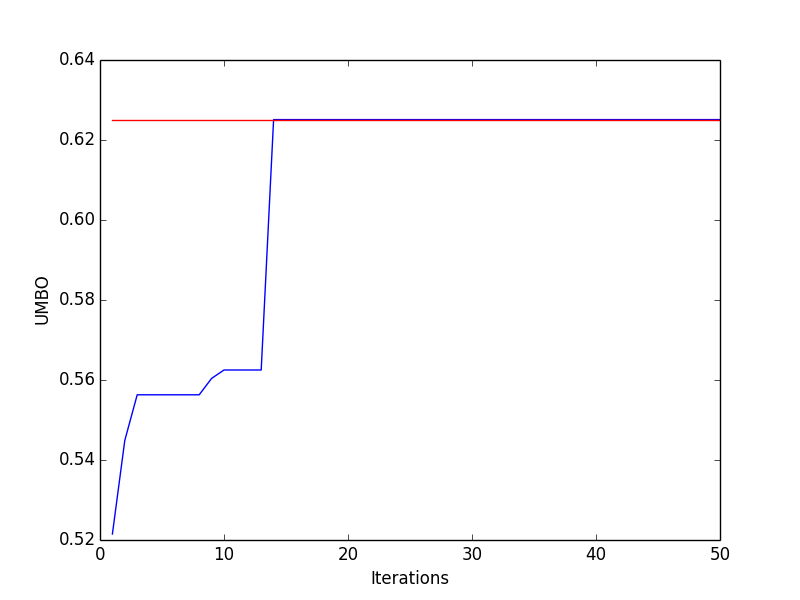
\includegraphics[scale=.8]{plot_BO_process.png}
\caption{Plot of the the maximum values by iteration}
\label{plot_bo}
\end{figure}
\end{center}
\section{Mixed-Halide Model}
\subsection{Model setup}
Let $V_x$ to denote the value of setup $x$. For each setup, there are three halides, one cation and a solvent. Since the positioning of the halides matters, there are in total 27*3*8 = 648 possible combinations. (i.e., $x\in\{1,...,648\}$). We use vector $Z^x$ to describe the components of setup $x$. In particular, $Z^x_i, i\in\{1,2,3\}$ is a binary variable that indicates which halide is in the 1st position. We require that $\sum_{i=1}^3Z^x_i=1, \forall x$. For example, $Z^x_{1,2,3} = (0,0,1)$ means that iodide is present in the 1st position. Likewise, $Z^x_i, i\in\{4,5,6\}$ is a binary variable that indicates which halide is present in the second position and $Z^x_i, i\in\{7,8,9\}$ in indicates which halide is present in the third position. $Z^x_{i}$, $i\in\{10,11,12\}$, indicates which cation is present in the setup. Again it is required that $\sum_{i=10}^{12}Z^x_i=1, \forall x$. $Z_{13}^x \in \{s_1,...,s_8\}$ indicates which solvent is used in setup $x$. In addition, for future computation, we let $s_i$ be a 2-d vector with the first entry being the MVEE and the second entry being the polarity of the $i^{th}$ solvent, $i\in\{1,...,8\}$. 

We still assume the presence of cations and halides contributes linearly to the value, and we use $\alpha_i$ to quantify the amount contributed by cation/halide $i$. To correct for the possible non-linear effect of cations and halides, we introduce $\beta_x$ for each of the setup x. For solvents, we assume they affect the UMBO through an unknown function $f:\mathbb{R}^{2}\mapsto \mathbb{R}$ which takes into consideration the MVEE and polarity of a solvent. Moreover, since a perovskite setup contains more than just a cation, a halide and a solvent, we use $\zeta$ to denote the invariant part of the setup. Hence UMBO of setup $x$ can be written in the following way:
\begin{equation}
V_x = \sum_{i=1}^{12}\alpha_i Z_i^x + \beta_x + \zeta + f(Z_{13}^x).
\end{equation}
We place the same prior distribution $N(\mu_{\alpha},\sigma^2_{\alpha})$ on each of $\alpha_i$, and $N(0, \sigma^2_{\beta})$ on $\beta_x$. $\zeta$ is assume to follow $N(\mu_{\zeta}, \sigma^2_{\zeta})$. We also view $f(\cdot)$ as a Gaussian process with prior $\mu_0(\cdot)$ and $\Sigma_0(\cdot,\cdot)$. Since $\zeta$ captures the invariant part of the setup, and somewhat a fixed amount to the solubility value, it is reasonable for us to assume $\mu_0(\cdot)=\mathbf{0}$. For $\Sigma_0(\cdot,\cdot)$, we use 5/2 Matern kernel. Let $r = \sqrt{\sum_{i=1}^{d}\ell_i(x_{1,i}-x_{2,i})^2}$ denote the distance between point $x_1$ and $x_2$ weighed by each dimension. In our case $d = 2$. The covariance between $x_1$ and $x_2$ under a 5/2 Matern kernel which is the same as the one described in section 1.

We place the same distributions on the parameters as in Section 1. We also use the same procedure described in section 1 to obtain prior parameters and to update posterior.
\subsection{single-sample batch} 
For single-sample batch, we select one point to sample in every batch. The computation of $EI$ and selection criterion for the next batch are the same as what has been described in section \ref{sec:sinEI}.
\subsection{multi-sample batch}
For multi-sample batch, we select $I$ points to sample in every batch. To be more precise, the batch-EI of $I$ points $x_1,...,x_I$ is defined as follows:
\begin{equation}
EI(x_1,...,x_I) = \mathbb{E}\left[(\max_{i\in\{1,...,I\}} V_i - f*)^+\Big|\mu_n,\Sigma_n\right]
\end{equation} 
An exact computation of the batch-EI is given in the paper \textit{Fast Computation of the Multi-points Expected
Improvement with Applications in Batch Selection} by Chevalier and Ginsbourger (https://hal.archives-ouvertes.fr/hal-00732512/document).
Let $b$ be the number of samples in a batch. We use the following algorithm to find the set $B = \argmax_{B\subseteq {1,...,N}}EI(B)$, with the cardinality of $B$ being $b$. (Recall $N$ is the total number of solutions.):
\begin{algorithm}
\caption{Algorithm for selecting $B$ sequentially}
\label{ag:B}
\begin{algorithmic}
\STATE $B := \{ \}$
\STATE $set = \{x_1,...,x_N\}$
\FOR{$i\in\{1,...,b\}$}
\STATE compute $x^* = \argmax_{i\in\{1,...,N\}}EI(B\cup\{x_i\})$
\STATE $B = batch \cup \{x^*\}$
\STATE $set = set\backslash \{x^*\}$
\ENDFOR
\end{algorithmic}
\end{algorithm}
The rest of the computation follows the same as the single-halide model.
\end{document}